\documentclass[11pt,a4paper]{scrbook}
\usepackage[utf8]{inputenc}
\usepackage[ngerman]{babel}
\usepackage{amsmath}
\usepackage{amsfonts}
\usepackage{amssymb}
\usepackage{blindtext}
\usepackage{graphicx}
\usepackage{url}
\usepackage[style=alphabetic-verb,backend=bibtex]{biblatex}
\bibliography{bibliografie}
\usepackage{listings}
\usepackage[hidelinks]{hyperref}
\usepackage{scrpage2}
\usepackage{csquotes}

\usepackage[right=2.5cm,left=1.5cm,top=3cm,bottom=2.8cm]{geometry}
\pagestyle{scrheadings}

\renewcommand\chapterheadstartvskip{\addvspace{-4ex}}


\linespread{1.5}

\clearpage

\newcommand{\q}[1]{``#1''}
\newcommand{\key}[1]{$[#1]$}


\begin{document}
\begin{titlepage}
\begin{center}

\vspace*{3cm}
\textbf{\huge{Projektarbeit}}\\
\vspace*{2cm}
\textbf{\large{Entwicklung eines 2D-Spiels mit SFML}}\\
\vspace*{5cm}
Gabriel Gavrilas, G3C\\
Jan Kunzmann, G3C\\
Patrick Eigensatz, G3C
\end{center}
\end{titlepage}


\clearpage
\thispagestyle{empty}
\clearpage\mbox{}\clearpage

\section*{Zusammenfassung}
Mit unserer Dokumentation wollen wir unsere Arbeitsweise, den zeitlichen Verlauf und die Funktionsweise unseres Projektes verdeutlichen.
Unser Projekt bestand aus dem Entwickeln eines 2D-Spiels.
Das Ziel des Spiels ist, als Einbrecher in ein Haus einzubrechen und dabei keinen Lärm zu verursachen und Laserschranken auszuweichen. Je nach Spielmodus hat man eine andere Aufgabe zu bewältigen.
Wir haben drei unterschiedliche Spielmodi vorgesehen:
\begin{itemize}
\item Zeitdruck: Innerhalb einer kurzen Zeit so viele Schätze wie möglich sammeln.
\item Sicherung: Die Schätze sind im ganzen Haus versteckt und gut mit Laserschranken gesichert.
\item Schatz: Es gibt je nach Level nur einen einzigen, im dunklen gut versteckten Schatz oder mehrere einfacher zu findende Schätze.
\end{itemize}
Zuerst gehen wir in dieser Dokumentation auf unsere Motivation, ein 2D-Spiel zu programmieren, ein.
Neben den allgemeinen Vorgaben, verdeutlichen wir auch unsere persönlichen Vorgaben.
Danach sind nochmal die im Projektvertrag aufgeführten Projektziele aufgelistet.
Die Definition der Begriffe und die Erläuterung der Entwicklungswerkzeuge sollten unseren Text verständlicher für Laien machen.
Sie stellen aber keinen Glossar dar, so können wir keine Vollständigkeit garantieren.
In Kapitel 5 ist der ganze Verlauf des Spieles dargestellt.
Die Erklärung der einzelnen Funktionen stellt auch die Entwicklung derer dar.
Da das Lösen von Problemen ein Hauptelement des Programmierens ist und unserer Arbeit war, haben wir uns die Zeit genommen, einige dieser Probleme zu erläutern.
Im Anhang finden sie noch den Quellcode zu unserem Projekt, welcher unser eigentliches Produkt darstellt.



\thispagestyle{empty}
\clearscrheadfoot
\lofoot[\pagemark]{\pagemark}
\refoot[\pagemark]{\pagemark}
\thispagestyle{empty}
\pagenumbering{gobble}
\tableofcontents

\clearpage
\pagenumbering{arabic}


\part{Dokumentation}
\chapter{Aufgabenstellung}
Wir haben die Aufgabe erhalten, während einem Semester eine Projektarbeit durchzuführen. Der Lernfortschritt wurde in einem Lernprotokoll laufend festgehalten.
Zum Schluss erstellten wir eine schriftliche Arbeit und eine Präsentation. Diese Arbeit soll uns auf die Maturarbeit vorbereiten.

\section{Motivation}
In unserer Generation verbringen viele Kinder, Jugendliche und Erwachsene ihre Zeit mit Computer- und Konsolenspielen.
Berühmte Vertreter sind zum Beispiel Call of Duty, Grand Theft Auto und Minecraft.
Doch die meisten Nutzer dieser Programme kennen die Prozesse und den Entwicklungsaufwand hinter diesen Games nicht.
Sei das auf Grund der weit fortgeschrittenen Komplexität einiger Spiele
oder bei simpleren Spielen die fehlende Motivation, sich damit zu befassen.\\
\\
Viele wollen nur wissen, wie man ein Spiel spielt und nicht, wie man es entwickelt. Nur wenige wissen, wie schwer und aufwändig es ist, bereits ein kleines Spiel herzustellen.
Da wir selber auch zu dieser Generation gehören,
gewinnen wir alle immer wieder Erfahrungen mit den verschiedensten Games.
Doch wir wollten nicht bloss Spiele spielen,
sondern wir wollten selber ein Spiel entwickeln.
Hinzu kam auch unsere Begeisterung für das Programmieren.
Jeder von uns hatte bereits ein wenig Erfahrung darin gesammelt.
Es hat jedoch noch niemand alleine
ein ganzes Game programmiert und
wir wollten und wollen stetig dazulernen.
Zusätzlich wollten wir am Ende dieser Arbeit etwas gemacht haben, das man auch nutzen kann.\\
\\
Wir möchten hier auch gleich die Gelegenheit nutzen und unserem Freund Mathias Rassasse danken. Er war ursprünglich auch Teil unserer Gruppe, er musste dann jedoch die Schule verlassen. Wir möchten ihm danken, weil er für uns die gesamte Musik zu unserem Spiel komponierte und einspielte.\\
\\
Ebenfalls bedanken möchten wir uns auch bei unserem Mentor, Herrn Sax. Er hat uns immer konstruktive Rückmeldungen und wertvolle Tipps geliefert, die uns weitergeholfen haben.


\section{Persönliche Vorgaben}

Vor dem eigentlichen Projekt setzten wir uns selber einige Vorgaben.
Uns war klar, dass ein Spiel auf dreidimensionaler Basis in der uns zu Verfügung stehenden Zeit nicht realisierbar sein würde. Deshalb entschieden wir uns für ein 2D Spiel.
Dazu brachte die von uns gewählte Programmiersprache einige Hilfen mit sich, die wir bei der Entwicklung eines 2D-Spiels gut gebrauchen konnten.
\\
Um die Sache für uns noch attraktiver zu machen, wählten wir bewusst eine Programmiersprache, die noch nicht alle von uns beherrschten.
Natürlich hätten wir genau so gut SDL oder direkt das darunterliegende OpenGL verwenden können.
OpenGL schied aber aus, da der Aufwand bereits ein einfaches 2D-Spiel zu realisieren zu gross gewesen wäre.
SDL war unser Favorit, bis wir SFML entdeckten.
Ganz im Gegensatz zu SDL ist SFML auf C++ ausgerichtet.
So wurden Klassen anstatt Strukturen verwendet, was den (für den
Anfang komplizierten) Umgang mit Zeigern reduzierte.
Ausserdem besitzen die Klassen eigene Konstruktoren, bzw. Destruktoren, was das Initialisieren
oder das Freigeben von Speicher überflüssig macht.
Davon erhofften wir uns weniger Speicherzugriffsfehler und ein schnelleres Programmieren.
SFML überzeugte uns schlussendlich, als wir die in der offiziellen Dokumentation gezeigten Beispielprogramme angeschaut hatten.

\section{Ziele}
\begin{itemize}
\item
Ziel unseres Projektes war es, ein 2D-Einbrecherspiel zu entwickeln. Der Spieler soll eine Figur spielen, die in Häuser einbrechen und dort unentdeckt Gegenstände entwenden soll.
\item
Ein persönliches Ziel war es, durch dieses Projekt die
Programmiersprache C++ zu lernen und zu vertiefen. Dies wollten wir nach dem Prinzip Learning-by-Doing erreichen. Jeder in der Gruppe sollte am Ende
C++-Programme selber programmieren können.
\item
Wir wollten
die Konzepte hinter Frameworks (namentlich SFML) verstehen und damit die
programmiertechnischen Abläufe hinter dem Spiel definieren und
umsetzen können.
\item
Wir beabsichtigten, unser Spiel komplett im Team zu entwickeln und
mit dem Versionskontrollsystem git vertraut werden. Das soll uns
auf spätere Projekte und unsere Maturarbeit vorbereiten.
\item
Das Spiel muss/soll unter eine OpenSource Lizenz gestellt werden.
\end{itemize}


\chapter{Begriffe}
\subparagraph{Game:}
In dieser Dokumentation werden wir öfters auch den englischen und weit verbreitete Begriff \q{Game} an der Stelle von \q{Spiel} gebrauchen.

\subparagraph{Multimedia Framework:}
Eine Bibliothek mit Funktionen, die sich in C++-Programme einbinden lassen. Damit kann man verschiedene Aufgaben plattformübergreifend bewältigen und muss nicht alle Details selber programmieren.

\subparagraph{OpenSource Lizenz:}

Eine Lizenz, die das Einsehen, das Verändern und das Weiterverteilen des Quellcodes erlaubt.

\subparagraph{OpenSource-Software (OSS):}
Software, die unter einer OpenSource-Lizenz verfügbar ist.

\subparagraph{Versionskontrollsystem:}
Ein Programm, das Veränderungen an Dateien aufzeichnet und speichert, sodass mehrere Entwickler den Code gleichzeitig ohne Redundanz verändern können.

\subparagraph{GitHub:}
Für OSS-Entwickler kostenlose Plattform, um die über das Versionskontrollsystem git aufgezeichneten Veränderungen übersichtlich zugänglich zu machen.

\subparagraph{Travis CI:}
Für OSS-Entwickler kostenlose Plattform zur Qualitätssicherung: Kompiliert das Projekt automatisch nach jeder Änderungen und führt Tests durch um sicherzustellen, dass das Programm einwandfrei funktioniert.

\subparagraph{Coverity:}
Für OSS-Entwickler kostenlose Plattform: Führt eine tiefgreifende statische Quellcodeanalyse durch, und hilft so Programmierfehler zu vermeiden und zu finden.

\chapter{Entwicklungswerkzeuge}
\section{Simple and Fast Multimedia Library}
\q{Simple and Fast Multimedia Library} (\textbf{SFML}) ist ein Multimediaframework, das wir hier als
\q{Entwicklungswerkzeug} einsetzen.
SFML liefert Klassen, die in verschiedenen Modulen (\textit{Sound}, \textit{Graphics}, \textit{Network}, ...) bereit stehen und aus dem Programm heraus aufgerufen oder im Programm verlinkt werden.
Diese Module wurden plattformübergreifend entwickelt. Deshalb mussten wir uns nicht um die Portierung unseres Spiels auf verschiedene Plattformen kümmern.
\\
\\
SFML stellt die Schnittstelle zwischen unserem Spielmodell im Arbeitsspeicher und dem Benutzer des Spiels bereit. Das Spielmodell verfolgt zum Beispiel den Standort der Spielfigur und SFML zeichnet eine entsprechende Bilddatei als Textur an die richtige Stelle auf den Bildschirm. Über SFML wird die Tastatur eingelesen und Musik abgespielt.

\section{Code::Blocks}
Code::Blocks ist eine frei verfügbare Entwicklungsumgebung (IDE\footnote{Integrated Development Environment}) zur Programmierung in C, C++ und D.
Neben der Syntaxhervorhebung und der intelligenten automatischen Code-Vervollständigung, bietet Code::Blocks bequeme Einstellungen um SFML-Projekte für mehrere Plattformen
komfortabel zu kompilieren. Code::Blocks setzt dabei auf eine Art \textbf{make}, wie es schon aus Unixzeiten bekannt ist: Neu kompiliert werden nur diejenigen Programmteile, welche sich
seit der letzten Kompilation geändert haben. Code::Blocks nutzt \textbf{g++}, den GNU C++ Compiler, um die einzelnen Dateien in Objektcode umzuwandeln und diese
anschliessend in einer ausführbaren Datei zusammenzuhängen (\q{linken}).

\section{git und GitHub}
\textbf{git} ist eine verteilte Dokument-Versionskontrolle (DVCS\footnote{Distributed Version Control System}). Ein solches Werkzeug hilft
den Entwicklern parallel zu programmieren und dabei die Übersicht zu behalten. Es zeichnet alle Änderungen am Code auf.  Diese kann man einsehen und zurückverfolgen, um Fehler zu finden und zu korrigieren. Es unterstützt auch die Wiederherstellung früherer Programmabschnitte, ohne dass man
manuell die Dateien zerpflücken muss. 
Git überzeugte uns durch seine Einfachheit, seine Effizienz und seine Möglichkeiten.
Git erwies sich als grosse Hilfe, sei es um Fehler zu finden oder einfach zum synchronisieren des Codes.
\\
\\
\textbf{GitHub} ist ein
Onlineportal, das das Hosting, also das Speichern von Projekten, die mit git verwaltet werden, kostenlos übernimmt. Das Projekt erhält eine eigene Übersichtseite,
die ebenfalls zur Entwicklung genutzt werden kann und auf der (fremde) Interessierte den Code und die Änderungen einsehen können. Wir haben GitHub nicht nur
als Hoster genutzt, sondern ebenfalls um unsere Termine im Projektkalender nachzuführen.
\begin{figure}
\centering
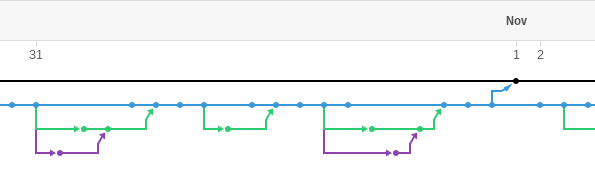
\includegraphics[scale=1]{img/branches.png}
\caption{Verschiedene Entwicklungszweige zur parallelen Entwicklung auf GitHub}
\label{fig:branches}
\end{figure}


\section{Coverity Scan}
\textbf{Coverity Scan} ist der Name eines Produktes der gleichnamigen amerikanischen Firma. 2006 erhielt diese Firma vom US-Verteidigungsministerium
einen finanziellen Zuschuss, um es für OpenSource-Projekte kostenlos möglich zu machen, ihren Code auf Sicherheitlücken und Programmierfehler untersuchen
zu lassen. Dabei funktioniert Coverity keineswegs wie ein normaler Compiler (erkennt also keine syntaktischen Fehler wie das Fehlen eines Semikolons),
sondern es versucht den Code zu verstehen und mögliche semantische Fehler zu finden. So werden Entwickler hingewiesen, dass zum Beispiel eine Funktion
unter gewissen Bedingungen nie terminiert wird und so das Programm blockiert wird. Auch findet Coverity schnell Speicherlecks und Speicherzugriffsfehler.
Während der Entwicklung haben wir unser Projekt regelmässig von Coverity überprüfen lassen.
\begin{figure}
\centering
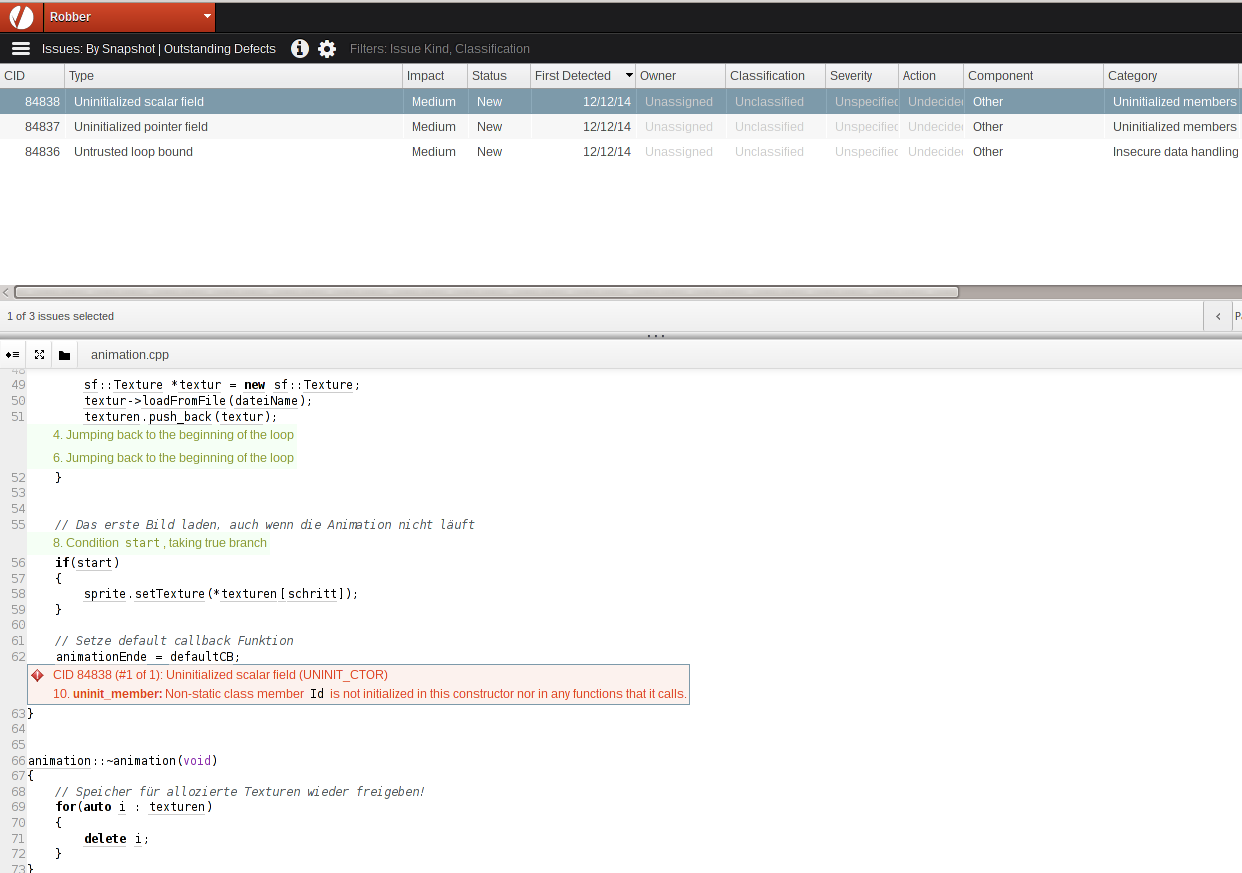
\includegraphics[scale=0.4]{img/coverity.png}
\caption{Coverity hat 3 Fehler gefunden und markiert die fehlerhafte Stelle im Code}
\end{figure}

\section{Valgrind}
\textbf{Valgrind} ist ein freies Programm zur dynamischen Fehleranalyse in Programmen. Besonders nutzten wir die Fähigkeit,
unser Spiel innerhalb Valgrinds Memcheck Modul laufen zu lassen, um ein Feedback über den Speicherverbrauch zu erhalten. So entdeckten
wir, dass viele Klassen, die schnell erstellt wurden, zwar Speicher anfordern, diesen aber nie mehr freigeben.
Das führte schlussendlich zu einem Speicherleck von knapp 20MB. Dies konnte dank Valgrind rasch festgestellt und behoben werden konnte.

\begin{figure}
\centering
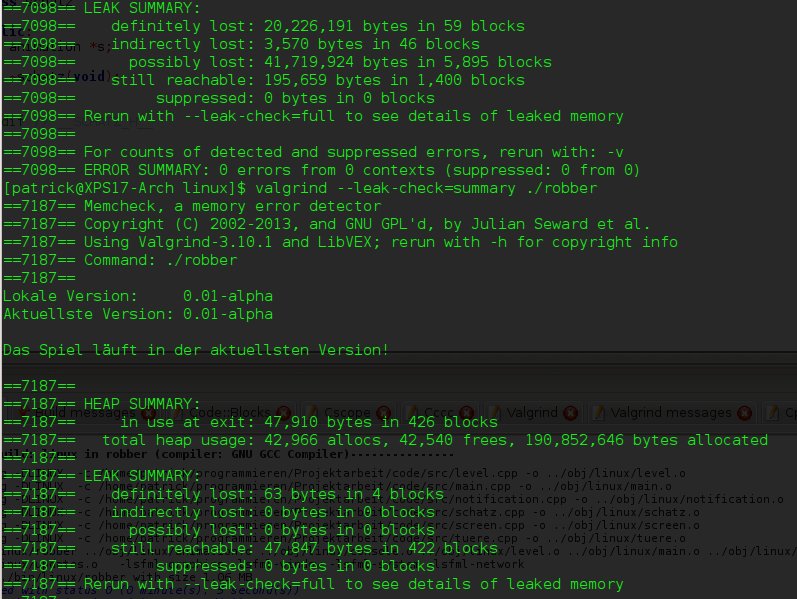
\includegraphics[scale=0.5]{img/valgrind2.png}
\caption{Valgrinds Memcheck Modul}
\end{figure}


\section{GIMP}
\textbf{GIMP} ist ein Programm zur Darstellung und Bearbeitung von Bilddateien.
Es stellt ähnliche Funktionen wie Photoshop zur Verfügung, ist jedoch kostenlos und frei verfügbar.
Wir nutzten GIMP zur Erstellung der Animationen und Grafiken unseres Spieles.
Dabei nutzten wir eine Vielzahl der bereitstehenden Funktionen von GIMP.
Alle Grafiken und Animationen unseres Spieles sind Eigenproduktionen oder entstammen den GIMP-Standardgrafiken.

\section{GDB - Der GNU Debugger}
Bei Fehlern, die sich in den Code einschlichen und zum Beispiel dazu führten, dass unser Spiel abstürzte, nutzten wir den GNU Debugger zur Problemfindung und Lösung. Ein Debugger lädt zunächst das Programm in eine gesicherte Umgebung. Dann wird das Programm Anweisung für Anweisung ausgeführt. Bei jedem Programmschritt kann der Programmierer genau betrachten, was das Programm macht und feststellen, wenn das Programm eine ungewollte Aktion ausführt. Ein Beispiel: Unser Spiel las einmal die Leveldatei falsch ein mit der Folge, dass das Spiel beim Laden hängen blieb und kurz danach abstürzte. Mithilfe des Debuggers konnten wir den Fehler eruieren und das Problem lösen. 

\chapter{Vorgehen}
\section{Vorbereitung}
\subsection{Spielidee}
Am Anfang stand die Ideenfindung auf unserer Agenda. 
Es war uns wichtig, eine Spielidee zu finden, an der ein Spieler über eine längere Zeit Spass haben würde.
Das Spiel sollte je nach unseren zeitlichen Möglichkeiten auch erweiterbar sein.
Folgende drei Fragen halfen uns bei der Wahl der Idee:
\begin{itemize}
\item Würdest du das Spiel spielen?
\item Ist das Spiel technisch überhaupt realisierbar?
\item Ist das Spiel erweiterbar?
\end{itemize}
Der Ideenfindungsprozess dauerte mehrere Wochen. Es war nicht einfach, eine Idee zu finden, die uns alle begeisterte.
Als wir Ideen gesammelt hatten, stellten wir eine Liste mit allen Ideen zusammen.
Wir setzten uns ein Frist von einer Woche, in der jeder von uns zu jeder Idee einen Umsetzungvorschlag erstellte.
Da wir drei Projektmitarbeitende waren, erhielten wir zu jeder Spielidee drei verschiedene Umsetzungvorschläge.
Nach längeren Diskussionen einigten wir uns schlussendlich auf die Idee des Einbrecherspiels:
Die Idee fanden wir alle interessant. Sie schien mit unseren Mitteln, unserem Wissen und innerhalb der zur Verfügung stehenden Zeit realisierbar zu sein. Und sie bot die Möglichkeit für spätere Erweiterungen.

\subsection{Vorbereitung und Planung}
Parallel zur Ideenfindung beschäftigten wir uns - wie in der
Disposition vermerkt - intensiv mit der Programmiersprache C++. Um C++ zu lernen verwendeten wir \cite{cpp_grundkurs}, um Sachen nachzuschlagen dienten uns aber auch \cite{cpp_referenz} und \cite{cpp_com}.\footnote{Infos zu den genannten Büchern finden Sie im Literaturverzeichnis} Das Einarbeiten in die Sprache war zentral für die spätere Verwendung der SFML-Bibliothek. In die SFML Bibliothek arbeiteten wir uns mithilfe der offiziellen Tutorials \cite{sfml_tutorials} ebenfalls sehr praxisorientiert ein.\\
\\
Die Reportage vom Schweizer Fernsehen \cite{sf_gamedesign} zum Thema Game Design halfen uns überhaupt nicht, da sie lediglich zwei Gamedesigner porträtierten und sie über ihre Motivation und ihren Studiengang Auskunft gaben, wir folglich daraus nichts für unsere Arbeit gewinnen konnten.\\
\\
Bevor wir nun jedoch mit der Programmierung anfangen konnten, mussten wir die Idee zu einem realisierbaren Konzept ausarbeiten.
Sicher war zuerst nur, dass es ein zweidimensionales Spiel sein würde und das Thema \q{Einbruch} werden sollte.
Der Einbruch in ein Haus und die Entwendung der Schätze sollten die Aufgaben sein, wobei wir 3 verschiedene Spielmodi planten:
\begin{itemize}
\item Einen bestimmten Gegenstand klauen
\item In einer bestimmten Zeit, so viel wie möglich stehlen
\item Einen möglichst hohen Wert an gestohlenen Waren erreichen
\end{itemize}
Wir entschieden uns für einfache Grafiken, um den Programmieraufwand gering zu halten. 
Bereits in diesem Stadium besprachen wir auch mögliche Problemfelder, auf die wir im Laufe des Projektes stossen könnten.
Beim skizzieren des Programms wurden die Grundsteine für wichtige Elemente unseres Programms gelegt: Kollisiondetektion (siehe Kapitel \ref{aufloesungsprobleme}, Teleportieren (siehe Kapitel \ref{Pfeile}), Schätze (Kapitel \ref{Schaetze}) oder auch die Architektur (Kapitel \ref{Loops}) auf der unser Spiel basiert.\\
\\
Durch die vorbeugende Fehlerantizipation konnten wir gewisse Probleme umgehen. Bei anderen mussten wir aber feststellen, dass einige Probleme komplexer waren, als wir ursprünglich dachten.
Der nächste Punkt war die Umsetzung des Konzeptes mit der Erstellung des Programms.

\subsection{Umsetzung}
Um die Planung während der Arbeit auch einzuhalten und voranzutreiben legten wir uns Stichtage fest, an denen wir gewisse Ziele erreicht haben wollten. Jeder wusste immer darüber Bescheid, welchen Stand das Projekt gerade hatte und was als nächstes zu tun war.\\
\\
Im Normalfall arbeiteten wir parallel, falls aber jemand auf Schwierigkeiten stiess, unterbrachen die anderen Projektmitarbeitenden ihre aktuellen Arbeiten und wir lösten das Problem gemeinsam.  
\newpage
\section{Einzelne Funktionen des Spiels}

\subsection{Überprüfung auf Updates}
Wir richteten auch eine Überprüfung auf Updates ein: Beim Start des Spiels lädt das Programm eine Versiondatei von GitHub herunter. Darin ist die Nummer der neusten Version des Spiels enthalten, mit der man dann überprüfen kann, ob eine aktuellere Version des Spiels verfügbar ist. Dementsprechend erscheint eine Meldung im Spiel.

\subsection{Kollisiondetektion}
Die Mauern der Häuser wollten wir direkt auf den Hintergrund zeichnen. Zu jeder Mauer erstellten wir ein Rechteck (FloatRect) mit dessen Koordinaten. Mit der Kollisiondetektion wird erkannt, ob die Koordinaten des Spielers in diesem Rechteck liegen.
Die Kollisionsdetektion war zu Beginn der Entwicklungen fehleranfällig.
Mehr zu diesen Fehlern wird im Kapitel \ref{mauern} auf der Seite \pageref{mauern} erläutert.
Das Prinzip der Kollisiondetektion der Mauern haben wir auf alle anderen Objekte wie Türen, Schätze und Laser übertragen.
Oft war die Kollisiondetektion bei diesen Objekten einfacher zu lösen, denn anstatt, der beim Erstellen des Levels abzumessenden Rechtecke, hatten wir bereits ein sogenanntes Sprite, welches die Lage und die Dimensionen des Objekts bestimmte.\\
\\
Meistens übergaben wir durch die Kollisionabfrage auch direkt einen Wert, welcher bei mehreren Objekten des gleichen Typs angab, welches Instanz des Objekts dieses Typs mit dem Spieler kollidiert.
Dadurch konnten wir mehrere Türen, Schätze und Laser implementieren.

\begin{figure}[h]
\centering
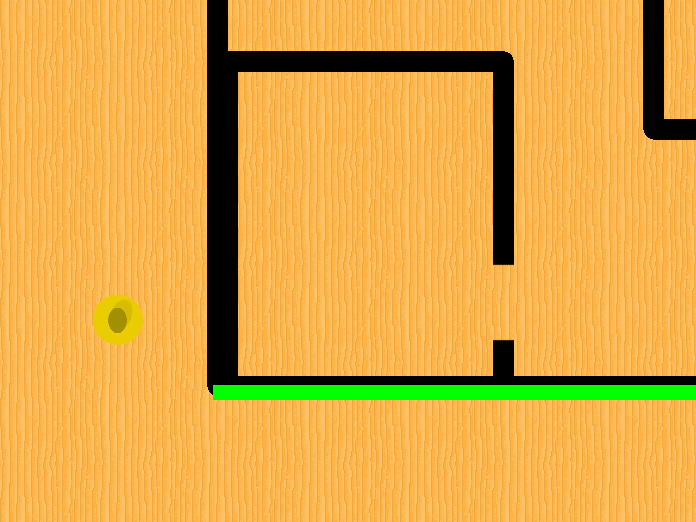
\includegraphics[scale=0.3]{img/kollisionsdetektion.png}
\caption{Debugging der Kollisionsdetektion}
\end{figure}

\subsection{Levelclass und Leveldatei}
Unser Absicht war es, zuerst ein Probe-Level zu erstellen. Daraus abgeleitet richtige Levels zu erstellen, schien uns das einfachste Vorgehen. 
Deshalb erstellten wir von Anbeginn zu jedem Level eine Leveldatei, in der alle variablen Informationen enthalten waren. 
Bei jedem Typ steht zuerst die Anzahl Objekte und zu jedem Objekt die genauen Koordinaten. 
Bei den Pfeilen wird zusätzlich die Position angegeben, an die der Spieler im neuen Level teleportiert werden soll. 
Zuerst definierten wir die Anzahl jedes Objektes, die es im entsprechenden Level hat und danach die benötigten Informationen zu den entsprechenden Objekten.
Das Programm liest nur Zahlen heraus anstelle von Beschreibungen. 
Den Mehraufwand, zum Einlesen von Wörtern aus der Leveldatei, sparten wir uns, um den Aufwand im Rahmen zu halten.

\begin{figure}[h]
\centering
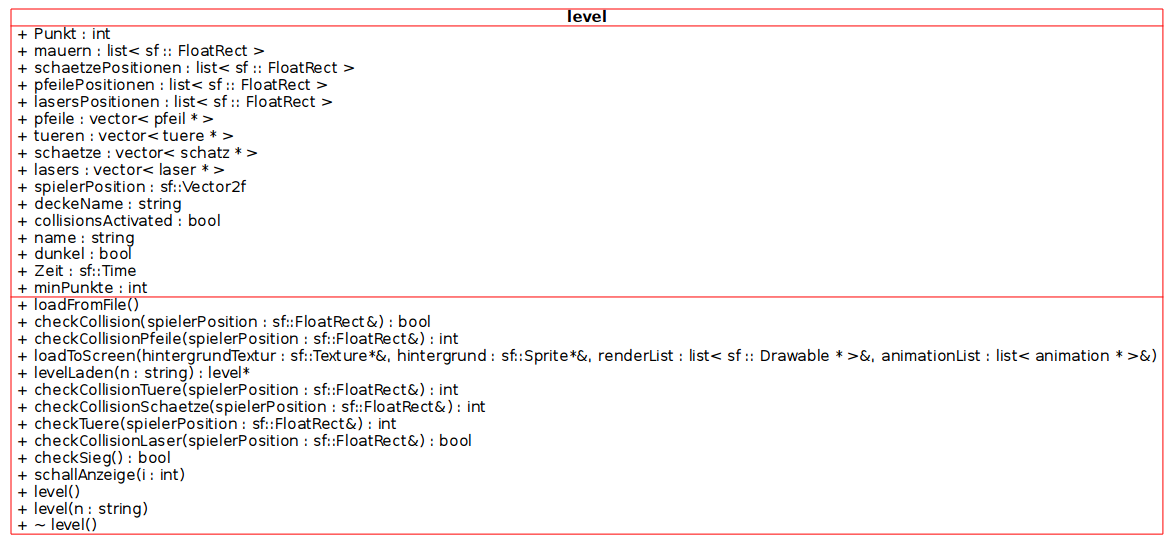
\includegraphics[scale=0.45]{img/level_uml.png}
\caption{UML der Levelklasse}
\end{figure}


\subsection{Animationen}
Von Anfang an waren Animationen in unserem Spiel eingeplant. So sollen zum Beispiel ausserhalb eines Hauses
Türen durch grün blinkende Pfeile markiert werden. Für solche Animationen wurde eigens eine Klasse implementiert.
\begin{figure}[h]
    \centering
    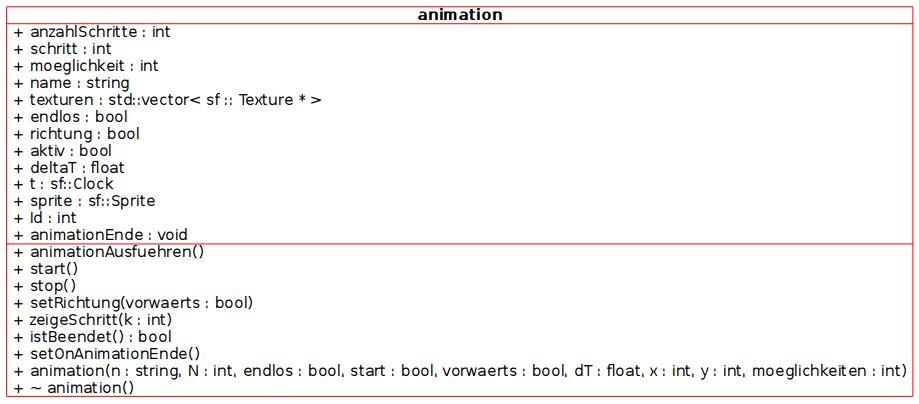
\includegraphics[scale=0.6]{img/animation_uml.png}
    \caption{UML der Animationsklasse}
\end{figure}
Um Animationen später oft und möglichst einfach verwenden zu können, besitzt die Klasse einen einfachen Konstruktor,
der die Bilder lädt, sowie die Position und die Zeitspanne $\Delta t$ zwischen den einzelnen Bildern festlegt.
Die Funktion zum Laden einer Animation hat viele Argumente, die viele verschiedene Animationen möglich macht. So gibt es neben der Zeitspanne auch die Option eine Animation endlos zu schalten oder diese rückwärts laufen zu lassen. Alle Objekte, ausserhalb den Mauern, bestehen aus einer Animation und optionalen Zusatzfunktionen.
\begin{figure}[h]
    \centering
    
\includegraphics[scale=0.3]{img/animation_pfeil.png}
    \caption{Die erste Animation im Spiel: Ein blinkender Einstiegspfeil}
\end{figure}
Innerhalb unserer $main()$-Funktion nützten wir eine $std::list<animation *>$ Liste aus der STL\footnote{Standard Template Library}.
Bevor die Sprites in das Fenster gezeichnet werden, werden die Texturen der Sprites dem Animationzeitpunkt entsprechend
neu geladen. So entsteht das Gefühl einer Bewegung oder eine Anpassung der Farbe. Entscheidend ist dabei die Methode
$animationAusfuehren()$, die überprüft, ob bereits genug Zeit vergangen ist, das neue Bild anzuzeigen und dies gegebenenfalls
übernimmt.


\subsection{Pfeile}
\label{Pfeile}
Anfangs nutzten wir einen Konsolenbefehl zum Wechseln der Level.
Um dies später auch dem Spieler zu ermöglichen, führten wir die Pfeile ein.
Die Pfeile erlauben dem Spieler das Eindringen in das Haus und die Flucht am Ende des Spieles.
In der Leveldatei geben wir das zu ladende Level an. Stösst man auf einen Pfeil, wechselt man zu diesem Level. In der Leveldatei geben wir die Anzahl Pfeile an. Darauf folgt ihr momentaner Standort und die Rotation. Durch zwei zusätzliche Zahlen wird die Startposition der Figur im neuen Level angegeben. Dies können wir später benutzen, um Häuser mit mehreren Etagen zu bilden.
Es gibt rote und grüne Pfeile. 
Die aktuelle Version des Spieles enthält bloss die grünen Pfeile.
In früheren Versionen gab es in den Levels, die den Garten darstellten, rote Pfeile.
Durch die Art des Levels konnten wir die Farbe der Pfeile steuern.
Unser Absicht ist es jedoch, beide Pfeile (rote und grüne) im gleichen Level laden zu können.
Darum gaben wir den Pfeilen eine weitere Variable mit, über die wir die Farbe jedes einzelnen Pfeils bestimmen können.
Rote Pfeile führen tiefer in den Level und grüne Pfeile aus dem Level hinaus.

\subsection{Console}
Wir haben eine Console eingebaut, die sich mit der rechten Shift-Taste öffnen lässt. 
In dieser kann man verschiedene kleine Hilfen aktivieren, 
wie zum Beispiel, dass man durch Mauern und Türen gehen kann (sogenannte Cheats). 
Über die Konsole kann man auch den Level direkt wechseln.
Die Konsole diente uns als Hilfe beim Testen des Spieles und wurde nicht für den Gebrauch für Spieler optimiert.

\subsection{Tastatur}
Die Figur wird mit den Tasten \key{W}, \key{A}, \key{S} und \key{D} bewegt. Mit der Taste \key{W} geht die Figur nach oben, mit \key{A} nach links, mit \key{S} nach unten, mit \key{D} nach rechts. Hier können wir im SFML auf eine einfache Funktion zurückgreifen. Diese erkennt, ob und welche Taste gedrückt wird. Jeder Taste ordneten wir einen bestimmten Befehl zu, der genau festlegt, was getan werden soll. Zum Beispiel steht bei der Taste \key{W}, dass sich die Figur um -5 Pixel bewegen soll. Dies bewirkt eine Bewegung nach oben. Da das Koordinatensystem bei jedem Laptop oben links mit 0/0 beginnt und dann nach oben und links negativ wird.\\
\\
Bei diesen Tastenabfragen wird auch gleich überprüft, ob man in eine Mauer läuft, sollte dies nämlich der Fall sein, darf sich die Figur nicht bewegen. Mehr dazu im ). 
Deshalb wird in diesem Fall der Schritt wieder rückgängig gemacht. 
Im Spiel kann man rennen. 
Dazu muss man die linke Shift Taste während der Bewegung gedrückt halten. Dann bewegt sich die Figur doppelt so schnell. Gleichzeitig wird der Schallpegel erhöht. 
Der Schallpegel wird auf Seite \pageref{Schall} erläutert.
Mit den Zahlentasten \key{9} und \key{0} kann man zoomen, um den Bildausschnitt um den Spieler herum zu vergrössern.\\
\\
Die Taste \key{E} hat mehrere Funktionen: Man kann damit einen Schatz aufnehmen. 
Durch eine Kollisionabfrage wird überprüft, ob der Spieler auf einem Schatz steht. 
Falls ja, verschwindet dieser vom Feld, indem er aus der $renderList$  wieder entfernt wird.\\
\\
Mit \key{E} lassen sich aber auch Türen öffnen. 
Auch hier findet eine Kollisionabfrage statt. 
Eine neue Animation kann erst nach dem Ende der vorangegangenen Animation neu gestartet werden. 
Sonst könnte man Türen schneller öffnen und schliessen, als es angezeigt würde. 
Wir haben das Rechteck um die virtuellen Türen etwas grösser definiert als deren Bild darstellt, damit die Figur auf dem Objekt \q{Türe} steht und sie mit dem Modul Kollisionabfrage öffnen und schliessen kann. Das Sprite wird für eine weitere Kollisionabfrage gebraucht, um zu verhindern, dass der Spieler ungehindert durch die Türen gehen kann, ohne diese zu öffnen. 
Dieses Konzept ermöglicht es, dass sich die Türen schlussendlich immer von beiden Seiten öffnen und schliessen lassen.


\subsection{Das Hauptmenü}     
Das Hauptmenü wurde bewusst einfach gehalten. Mit GIMP wurden     
einige Grafiken erzeugt, die als Schaltflächen verwendet werden.
Zuerst versuchten wir, das Hauptmenü als festes Bild anzuzeigen. Doch wir stiessen dabei auf Auflösungprobleme (Siehe Seite: \pageref{aufloesungsprobleme}).
Schlussendlich erstellten wir einen speziellen Hauptmenülevel.
Man beginnt nun direkt mit dem Spieler.
Dadurch setzen wir die Spielfigur als zentrales Element des Spieles auch im Hauptmenü ein.
Wir definierten das Bild mit der Textur \q{Spiel starten} als neuen Pfeiltyp. 
Zur Definition dieses Pfeils übergeben wir seiner Farbe die Zahl 2. 
Sobald man auf das \q{Spiel starten} fährt, wird man in den Garten des ersten Hauses teleportiert. 
Um das Spiel zu beenden, fährt man mit dem Spieler über das \q{Spiel beenden}. Mit der Kollisiondetektion erkennt man diese Aktion und das Spiel wird beendet.

\subsection{Musik}     
Alle Elemente unseres Spiels wollten wir in grösstmöglicher Eigenproduktion erstellen. Für die Musik baten wir unseren gemeinsamen Freund Mathias Rassasse, welcher die nötigen Mittel hat, unsere Musik zu komponieren und einzuspielen. Verdankenswerterweise folgte er unserem Wunsch und stellte uns die Musik mit unbeschränktem Nutzungsrecht zur Verfügung. 
Seine Musik wird nun im Hintergrund während des Spiels abgespielt. 
Für die Musik hat SFML eine eigene Klasse. 
Insgesamt bauten wir 3 Musikstücke ins Game ein. 
Eines für das Hauptmenü, eines für die Levels und das Letzte für das Game Over. 
Das Abspielen der Musikstücke zum richtigen Zeitpunkt während des Spiels lösten wir so, dass wir den Namen der Leveldatei überprüfen und je nach Namen, die zugehörige Musik abspielen.
    
    
\subsection{Dunkle Level}     
Mit einem halbtransparenten Overlay können wir das Level, bzw. das Haus, abdunkeln und nur in einem Bereich um den Spieler sichtbar machen.
In der Leveldatei wird eingetragen, ob ein Level dunkel oder hell ist. Dementsprechend wird dann das Overlay geladen oder eben nicht. Das führt zu einem spannenderen Spiel. Denn man erkennt die Gefahren und die Schätze erst später, wenn man sich durch den Level durchgetastet hat.
Besonders beim Spiel auf Zeit entsteht so ein zusätzlicher Druck. 

\begin{figure}[h]     
\centering     
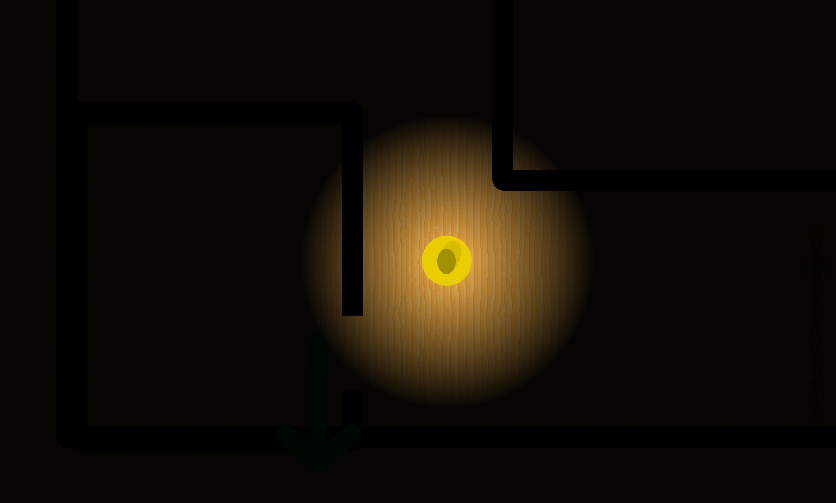
\includegraphics[scale=0.5]{img/dunkel.png}     
\caption{Ein dunkles Level}     
\end{figure}         
    
\subsection{Schallpegel}
\label{Schall}      
Um den Spieler zu zwingen, sich auch wie ein Einbrecher zu verhalten, haben wir einen Schallpegel eingeführt. Es gibt momentan zwei Methoden Lärm zu machen.
Entweder man öffnet oder schliesst eine Türe oder man rennt. 
Dadurch wird jeweils eine bestimmte Zahl zum Schallpegel addiert.
Laufend wird jedoch auch ein konstanter Wert wieder abgezogen, so sinkt der Schallpegel ständig.
Links auf dem Bildschirm haben wir eine Anzeige erstellt, die den aktuellen Schallpegel anzeigt.
Diese Anzeige ist eine Animation, welche für jeden Zehnerwert der Schallanzeige ein eigenes Bild hat.
Sobald diese den roten Bereich erreicht, riskiert man wegen zu vielem Lärm das Spiel zu verlieren.
Um dem Spieler im roten Bereich doch noch eine Chance zu geben, bauten wir eine Zufallszahl ein.
Diese Zahl liegt zwischen 1 und 200. 
Der Zufallswert wird bei jedem Durchgang des Codes neu berechnet.
Wenn diese Zahl einmal den Wert 199 hat, verliert man das Spiel und kommt in das \q{Game Over}-Level.
Der Schallpegel existiert nur in den dunklen Levels, denn nur dort muss man leise sein.

\subsection{Schätze und Punkte}
\label{Schaetze}
Das Ziel des Spieles ist es, alle oder eine bestimmte Anzahl an Schätzen eines Levels zu stehlen.
Die Schätze bestehen aus einer Animation, welche nur einmal ausgeführt werden kann.
Zusätzlich gibt es zwei mögliche Schatztexturen, welche durch eine Funktion in der Animationsklasse zufällig ausgewählt werden.
Sobald man die Animation ausführt verschwindet der Schatz.
\\
Um diesen Schätzen einen Wert zu geben, haben wir ein Punktesystem eingeführt.
Für jeden Schatz erhält man zehn Punkte, welche oben links angezeigt werden.
In der Leveldatei haben wir für jeden Level einen Mindestwert an Punkten festgelegt, der erreicht werden muss.
Bei Erreichung der Mindestanzahl an Punkten, startet die $sieg()$-Funktion.
In der momentanen Programm-Version dieser Funktion, gerät man direkt in das Hauptmenü.
Ihr eigentlicher Sinn wäre es aber (spätere Programmerweiterung, direkt den Weg in den nächste Level zu öffnen, sei das durch direkte Teleportation oder durch Freischalten eines Pfeils.    

\subsection{Laser}
Das Schwierigkeit, in einem dunklen Level zu rennen, ist neben der Zeit auch die Gefahr, mit einem Laser zu kollidieren.
Die Laser bilden Hindernisse auf dem Weg zu den Schätzen.
Um die Laser in unserem zweidimensionalen Spiel passierbar zu machen, lassen wir sie pulsieren.
Sobald die Animation keinen durchgehenden Laser anzeigt, ist die Laserschranke passierbar.
Sobald sie jedoch wieder leuchtet, verliert man bei einer Kollision das Spiel.
\\
Die Idee der Laserschranken ist ein Alarmsystem, welches bei einer Unterbrechung des Lasers Alarm schlägt. In Verbindung mit zukünftigen Gegenspieler könnte die Alarmanlage den Schallpegel auf den höchsten Wert setzen und damit alle Gegenspieler aufwecken.

\subsection{Zeit}
\label{Zeitlimit}
Zusätzlich zu den Lasern und zum Schallpegel führten wir die Zeit als erschwerdender Faktor ein. 
So zählt eine Anzeige im Spielbildschirm oben links in Sekunden von einem vorgegebenen Startwert herunter. Falls man das Level nicht vor dem Enden der Zeit verlassen hat, verliert man das Spiel und geht GameOver. Die zur Verfügung stehende Zeit ist pro Level variabel wählbar. Deshalb wird sie in der Leveldatei angegeben.
    

\section{Wahl der Spielarchitektur}
Als wir die Grundlagen von C++ zusammen erarbeitet hatten, planten wir das Vorgehen zur Programmierung des Spiels.
Wir kannten zwar Verzweigungen, Schleifen und Funktionen, aber \q{wie können wir damit ein Spiel entwickeln?} Auf Seite 106 in \cite{sfml_gamedev}
wird eine parallele Spielarchitektur erklärt. Wir fanden diese aber unnötig kompliziert. Deshalb erarbeiteten wir uns eine eigene andere Struktur. Daraus resultierte die Struktur in Abbildung \ref{fig:seriell}.\\
\begin{figure}[h]
\centering
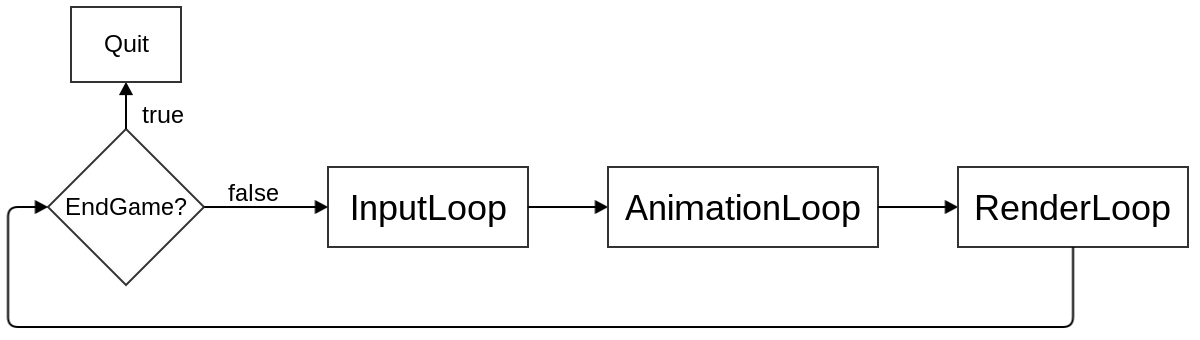
\includegraphics[scale=0.3]{img/gameloops.png}
\caption{Unsere serielle Spielarchitektur}
\label{fig:seriell}
\end{figure}

\subsection{Serielle Architektur}
\label{Loops}
Die serielle Architektur unterteilt sich in vier Teile, die immer vollständig und immer hintereinander ablaufen. Die Funktionsweise
und die Aufgaben der Teile werden hier kurz erläutert:\\
\\
\textbf{EndGame?}
Diese Abfrage überprüft nur, ob das Spiel beendet werden muss, sei es aufgrund eines Fehlers im Spiel
oder weil der Benutzer das Fenster schliessen wollte.\\
\\
\textbf{InputLoop}
Dieser Teil ist dafür zuständig, die Eingaben des Spielers einzulesen und aufgrund der Eingaben Aktionen auszulösen. Die Aktionen lösen Änderungen am Levelmodell im Speicher aus und wirken sich somit zum Beispiel auf die Position des Spielers, einer Türe oder auf die Punkte aus. 
\\
\textbf{AnimationLoop}
In der AnimationLoop wird für jede Animation überprüft, ob sie aktiv ist, und wenn ja, ob seit dem letzten Durchgang bereits die für jede Animation
eigene Zeit $\Delta t$ verstrichen ist, damit dem Sprite die nächste Textur zugeordnet werden kann.\\
\\
\textbf{RenderLoop}
Die einzelnen Sprites werden in das SFML-Fenster gezeichnet, und SFML wird angewiesen das Fenster neu auf den Bildschirm zu \q{zeichnen}.

\subsection{Parallele Architektur}
SFML unterstüzt mit der \textit{Thread}-Klasse eine plattformübergreifende Implementierung
von Systemthreads. Wenn ein Thread erstellt wird, springt das Programm an diesem Punkt
in eine Funktion und führt diese parallel zum Rest des Programms aus. Der Vorteil,
der sich dadurch ergibt, ist die Performancesteigerung, d.h. die Ausführungsgeschwindigkeit des Programms. Die
parallele Architektur würde sich demnach in drei bis vier Teile aufgabeln. Je nachdem, ob man die AnimationLoop
und die RenderLoop in jeweils einzelne Threads nimmt oder nicht. Da wir zu Beginn
nicht wussten, dass SFML so effizient arbeiten würde, und unser Spiel auch ohne parallelen Code
ohne Ruckler spielbar wäre, hatten wir unsere Spielarchitektur ursprünglich nur parallel geplant:
\\
\begin{figure}[h]
\centering
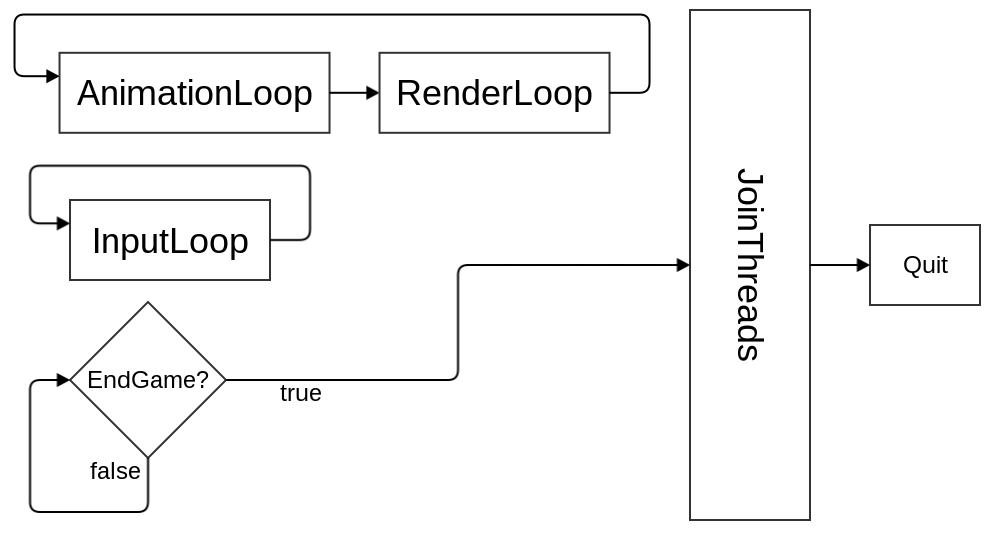
\includegraphics[scale=0.3]{img/threads.png}
\caption{Die parallele Spielarchitektur}
\end{figure}


\chapter{Herausforderungen und Lösungen}     
\section{Auflösungsprobleme}     
\label{aufloesungsprobleme}
Schon früh im Projekt zeigte sich ein Problem beim Abspielen des Games mit verschiedenen Computern mit unterschiedlichen Bildschirmauflösungen. Es stellte sich heraus, dass es sich
beim Auflösungsproblem um ein Problem beim Umgang mit SFML handelte.
Die Herausforderung bestand darin, dass jede Ansicht des Games bei jeder Auflösung, jeder Gerätemarke und bei beiden Betriebssystemen gleich aussehen sollte.
Wir hofften, dass SFML diese Arbeit übernehmen würde, doch bereits bei den ersten Grafiken stellten wir fest, dass wir die Anforderung selber regeln müssen.
Um die Aufgabe zu lösen, benutzten wir die $zoom()$-Funktion, mit der die Grösse der ganzen Ansicht über einen Wert angepasst werden kann.
Diesen Wert nannten wir factor.
Diesen factor bestimmten wir durch den Quotienten aus Auflösung und Ansichtsgrösse.
\begin{quote}
Eine View ist eine Klasse der SFML Bibliothek.
Man kann es sich als eine 2D-Kamera vorstellen, die definiert, welche Region des Bildes angezeigt wird.
Wir haben die View für unser Spiel Ansicht genannt.
\end{quote}
Wir erhofften uns, durch Einsetzen verschiedener Werte des factors, eine Gesätzmässigkeit zu finden.
Schnell wurde uns jedoch bewusst, dass diese Lösung längerfristig nicht haltbar war. 
Denn dies führte auch dazu, dass zum Beispiel die Mauern umgerechnet werden mussten.
Nicht nur war der geschätzte Aufwand sehr gross, sondern dieser Ansatz hätte weitere Probleme mit sich gebracht.
\\
\label{mauern}
Bei den ersten Mauern waren die FloatRect der Mauern zu Beginn je nach Position auf dem Spielfeld unterschiedlich und falsch.
Es gab vereinzelt Schlupflöcher von ganz geringer Breite, sodass man durch die Mauer hindurch konnte. 
Neben der Mauer hingegen, versteckte sich eine unsichtbare Mauer. 
Das heisst, es wurde eine Kollision mit einer Mauer gemeldet, obwohl an der Spielerposition gar keine Mauer eingezeichnet war. 
Um das Problem zu erforschen und schliesslich zu beheben, ladeten
wir die Mauerabschnitte einzeln und zeichneten grüne Rechtecke darüber. 
Auf diese Weise entdeckten wir, dass die Koordinaten der Mauer zwar richtig eingelesen, aber falsch verarbeitet wurden. Die Lösung war: Die Koordinaten mussten
von absoluten Bildschirmkoordinaten in Fenster/Spielkoordinaten umgerechnet werden. 
Durch weitere Tests konnten wir den factor so verändern, dass keine Fehler mehr auftraten. 
Weitere Versuche zeigten leider, dass die Mauern im Allgemeinen aber immer noch nicht richtig verrechnet wurden.
Schlussendlich mussten wir einsehen, dass das Problem mit dem gewählten Vorgehen nicht gelöst werden konnte.\\
\\
Das Problem war die Handhabung von drei verschiedenen Koordinatensystemen.
SFML regelt seine Grafiken mit zwei Koordinatensystemen.
Das erste hatte das Zentrum in der linken oberen Ecke des Bildschirms und gibt jedem Pixel des Bildschirms eine Koordinate.
Die Ansicht ist an dieses System gebunden.
Das zweite System hat seinen Zentrum in der virtuellen oberen linken Ecken der Grafiken.
Von dort werden die Positionen der Grafiken innerhalb des Fensters bestimmt.
Dieses System ist frei von der Ansicht. Sie kann sich frei über dieses System bewegen.
Über vordefinierte Funktionen der SFML Bibliothek rechneten wir die Koordinaten zwischen den Systemen ineinander um.
Wir selber erstellten mit dem factor ein eigenes, neues System.
Wir brauchten viel Zeit zum Verstehen der Zusammenhänge dieser drei Koordinatensysteme.\\
\\

Durch das Verankern der Ansicht an den Spieler, konnten wir die Arbeit mit dem factor umgehen und ihn wieder herausstreichen.
Diese Variante gefiel uns besser, denn wir gingen nie von immer gleich grossen Levels aus. 
Das wäre beim factor ein weiteres grosses Problem geworden.
\\
Wie bereits erwähnt regelt SFML das Anzeigen mit zwei Koordinatensystemen. Wir entdeckten einerseits einen Fehler bei der Bestimmung der Auflösung des Bildschirms und andererseits in der Anpassung der Grafiken an die gemessene Auflösung im Spiel.
Dadurch kam und kommt es auf wenigen Bildschirmen mit hoher Auflösung immer noch zu Anzeigefehler. Wir griffen auf die SFML \textit{zoom()}-Funktion zurück, um den Wert während des Spiels manipulierbar zu machen. So sieht man zwar am Anfang den Fehler, kann ihn aber durch zoomen mit den Tasten \key{0} und \key{9} irrelevant machen.

Wir können weitere Fehler bei dieser Funktion nicht ausschliessen, doch haben wir uns entschlossen, dieses Thema aus Zeitgründen nicht weiter zu verfolgen. 

\section{Compilerprobleme}
Nicht nur wir machten Fehler bei der Entwicklung, sondern offenbar auch die Entwickler unseres Compilers. Wohlbemerkt, dass die Fehler von anderen erfahrungsgemäss schwerer aufzuspüren sind!\\
\\
Einem eher speziellen Problem begegneten wir, als wir den Pfad für ein Animationsbild erstellen wollten.
Die Zahl $i$, die bei 0 zu zählen anfängt, zeigt, den wievielten Schritt der Animation gerade geladen werden soll, und $n$ steht für den Namen der Animation.
Ein solcher Pfad lautet zum Beispiel für einen\\Pfeil im 4. Animationsschritt: \textit{resources/pfeil\_3.png}\\
\\
In C++11 sind die + Operatoren zur Verkettung (Engl. concatenate) von Strings überladen. Damit man auch Zahlen in Strings einsetzen
kann, gibt es seit C++11 die Funktion $to\_string()$, die überladen für sämtliche Zahldatentypen existiert und das Argument in einen String
umwandelt. Der Code kompilierte auf Linux mit dem GNU C++ Compiler (G++) v4.9 ohne Probleme. Als Gabriel und Jan versuchten den Code auf ihrem Windowssystemen
mit dem für Windows aktuellen MinGW G++ v4.7.1 zu kompilieren scheiterte dies. Spannende Recherchen ergaben, dass es sich um einen bei MinGW gemeldeten Bug\footnote{\url{https://gcc.gnu.org/bugzilla/show_bug.cgi?id=52015}} handelt, der ein Auffinden der Funktion in der unter Windows verwendeten
Version unmöglich macht. Glaubt man den Kommentaren zum Bug, so findet der Präprozessor den Header zwar, liest ihn aber auf Grund eines Guardtokens nicht ein.
Die Funktion ist folglich in der libc++ implementiert, wird aber in keinem Header deklariert.\\ %nur leicht unklar für unwissende...
\\
Ein Lösungsansatz wäre gewesen, die in C für diesen Zweck bestimmte Funktion \textit{sprintf()} zu nutzen, dies hätte jedoch einen C-String zur Folge gehabt.
Da wir am Anfang C++ als Programmiersprache wählten, um den C-Problemen wie Speicherverwaltung, C-Strings, etc. aus dem Weg zu gehen, entschieden wir uns, über ein
Präprozessorflag (\textit{\#ifndef}) das \textit{LINUX}-Makro zu prüfen. Existiert dieses, so wird die to\_string()-Funktion, ansonsten ein stringstream, verwendet.
Der Commit \textit{e419eef} behebt und dokumentiert genau dieses Problem. Um uns auch später, also während der Erstellung der Dokumentation, einen Überblick
über die behandelten Probleme verschaffen zu können, haben wir diese in den Commits jeweils kurz erläutert. Das genannte Problem findet sich im
Konstruktor der Animationsklasse, in der Datei \textit{code/src/animation.cpp}.

\begin{figure}[h]
\centering
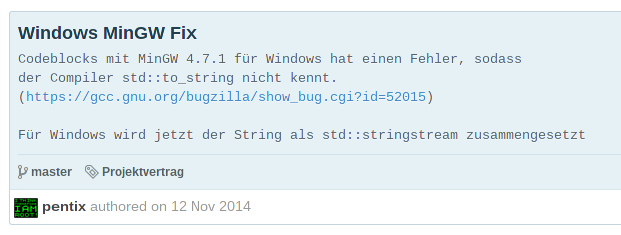
\includegraphics[scale=0.8]{img/e419eef.png}
\caption{Erläuterung in einem Commit}
\end{figure}

\section{Fehler in der Leveldatei}
Jeder spielbare Level wird, wie bereits erläutert, aus einer Leveldatei geladen.
Das Erstellen einer solchen ist mit viel Aufwand verbunden, denn sie muss genau auf die Levelclass abgestimmt sein.
Beim Erstellen, oder durch Vernachlässigung einiger Dateien nach dem Bearbeiten der Levelclass, kann es zu Fehlern kommen.
Die meisten Grafikfehler gehen auf diese Art von Fehlern zurück.
Dabei kann das Spiel die Datei zwar lesen, gibt aber einen Fehler aus: \q{Fehler beim Laden der Leveldatei: } und den entsprechenden Levelnamen.


\section{Doppelter Tastendruck}
Bei der Implementierung der Schätze, stellten wir fest, dass SFML ein Problem mit der Anzahl Anschläge von Tasten hat.
So kam es zu doppelten Punkten beim einsammeln von Schätzen.
Auch bei den Türen traten gleiche Probleme auf. Durch das Bestimmen der Animationslänge und des Animationsstartverbotes während der Animation konnte der Fehler bei den Türen aufgehoben wurden.
Bei den Schätzen lösten wir es mit einer internen Uhr, deren einzige Funktion eine Verzögerung ist, so dass ein Schatz erst bei wirklich erneutem Drücken der Taste aufgenommen wird.


\section{Merge Conflicts}
Git, unsere Versionskontrolle, ermöglichte es uns, parallel, in sogenannten Branches zu entwickeln. (Siehe Abbildung \ref{fig:branches} auf Seite \pageref{fig:branches}). Wir entwickelten neue Funktionen oft parallel und \q{mergten} (engl. to merge = zusammenführen) sie in unseren master-Zweig.
git übernimmt alle Änderungen, die in beiden Zweigen seit dem letzten gemeinsamen Commit erstellt wurden, und erstellt daraus neue Dateien, die alle Änderungen,
also die Änderungen von beiden Zweigen beeinhalten. Es kann sein, dass nun 2 Personen gleichzeitig an derselben Stelle im Code etwas geändert haben. Zum Beispiel
hat der eine Entwickler eine Abfrage gelöscht, weil er sie nicht mehr brauchte, ein anderer Entwickler hat jedoch dieselbe Abfrage erweitert, da er sie benötigt.
Git kann nun nicht mehr automatisch entscheiden wie der Code zusammenzuführen ist, bzw. wie die beiden Versionen kombiniert werden sollen. Daraus resultiert ein Merge
Conflict. Git erstellt eine Datei, in der beide Versionen der Entwickler vorhanden sind und bittet den Entwickler, der den Code des anderen in seinen zusammenführen
will, um Hilfe. Unsere Konflikte waren meistens schnell gelöst, da sie jeweils nur zwei bis drei Zeilen betrafen. Zum Beispiel wurde bei beiden Entwicklern
eine Variable unbenannt und man musste entscheiden, welche Variabel man wählt.\\
\\
Mühsam hingegen waren Konflikte, die mehrere Dateien betrafen und in der 20 bis 30 Zeilen in einem Klammerwirrwar im Konflikt standen. Da die Dateien und die Zeilen
logisch voneinander abhängen, musste man sehr vorsichtig sein. Man brauchte entsprechend viel Zeit und Geduld einen solchen Konflikt zu lösen. Es gab zum Glück keinen
grossen Konflikt, der uns grosse Probleme bereitete.

\section{Paralleles Entwickeln des Kerns}
Obwohl wir bereits am Anfang hätten parallel mit git entwickeln können, gelang uns dies nicht von Anbeginn. Der Start war sehr schwierig, da noch gar kein Code vorhanden war
und es zuerst galt eine Basis zu entwickeln, auf der dann alle programmieren konnten. Wir versuchten von Anfang an so zu programmieren,
dass wir später keine grossen Änderungen vornehmen mussten, wenn das Spiel um verschiedene Funktionen wie Laserschranken oder auch Musik erweitert werden sollte.
\\
\\
Das gelang uns generell sehr gut. Einzig die Levelklasse brauchten eine Restrukturierung, weil die \textit{loadFromFile()}-Methode eine Leveldatei nicht nur auslas,
sondern die Objekte auch gleich zeichnete. Da wir die Level aber speichern und nicht immer komplett neu laden wollten, brauchten wir eine
Funktion, die es uns ermöglichte, nur die Objekte in die Levelklasse zu laden und eine Funktion, die nur die gespeicherten Objekte zeichnete. So konnten wir Veränderungen an den Objekten in der Levelklasse abspeichern.
\\
\\
Ansonsten mussten wir am ganzen Kern nichts mehr ändern. Dadurch ergab sich der grosse Vorteil, dass jeder Programmierer seine
Funktionen bestens kannte und problemlos Objekte erstellen konnte, welche auch auf Kollisionen mit dem Spieler geprüft werden konnte.

\section{Mathematik}
Das Überthema unserer Projektunterricht-Kursgruppe ist Mathematik im Alltag.
Passend dazu hatten wir uns mit vielen mathematischen und logischen Problemen beim Programmieren auseinanderzusetzen.
Programmieren selber ist ein sehr Logik-gebundener Prozess.
Einfache Beispiele sind logische Verknüpfungen oder Bedingungen.
Doch meisten sind es komplexere Probleme, wie zum Beispiel das Regeln von Unterordnungen oder das korrekte Aufrufen von definierten Variablen.
Auch das Auflösungsproblem gehört zu dieser Art von Problemen.
\\
Ein weiteres Beispiel für logische Probleme sind die Türen.
Uns war es wichtig, dass die Türen nach dem Aufmachen und Zumachen jeweils unpassierbar sind.
Dazu mussten wir eine Funktion definieren, die am Ende der jeweiligen Animation aufgerufen wird und eine Mauer erstellt.
Das Problem hierbei war das Regeln der verschieden Klassen.
Durch Probieren und vielem Nachdenken kamen wir auf die Idee Funktionspointer zu gebrauchen.
(Die ausführliche Problemerläuterung kann im Lernprotokoll nachgelesen werden.)
\\
Zu den logischen Problemen beim Programmieren kamen auch einfach arithmetische und geometrische Probleme.
So hatten wir Mühe beim Berechnen der Mauerkoordinaten für die Türe bei jeder möglichen Rotation, wobei wir uns auf neunzig Grad Drehungen beschränkten.
Zum Schluss gab es auch noch Fehler, die durch die Komplexität des Codes entstanden.
Beim Erstellen eines weiteren Testlevels, der mehrere Laser haben sollte, kam es zu Fehlern.
Es wurden zwar alle Laser angezeigt, doch nur ein Laser funktionierte.
Sie wurden zwar gezeichnet, aber die Kollisionabfrage gab keine Kollision aus.
Nach tiefschürfender Programmcodeanalyse fiel uns auf, dass immer nur der erste Laser funktionierte. Da wurde uns klar, dass der return-Befehl innerhalb der verschachtelten Abfragen eine Abfrage zu früh ausgeführt wurde. Nach dem Korrigieren wurden alle Laser richtig eingelesen und verarbeitet.



\section{Verfügbare Zeit}
Am Anfang des Projektunterrichts dachten wir, wir hätten mehr Zeit für die eigentliche Entwicklung. Wir mussten schlussendlich aber auch
sehr viel Zeit in die Disposition, den Projektvertrag und das Lernprotokoll stecken. Die Zeit, die uns für die Dokumentation und das Spiel
blieb, nutzten wir aber sehr intensiv. Die Kreise in Abbildung \ref{fig:punchcard} zeigen additiv, wie viel und wann seit Projektbeginn programmiert wurde.

\begin{figure}[h]
\centering
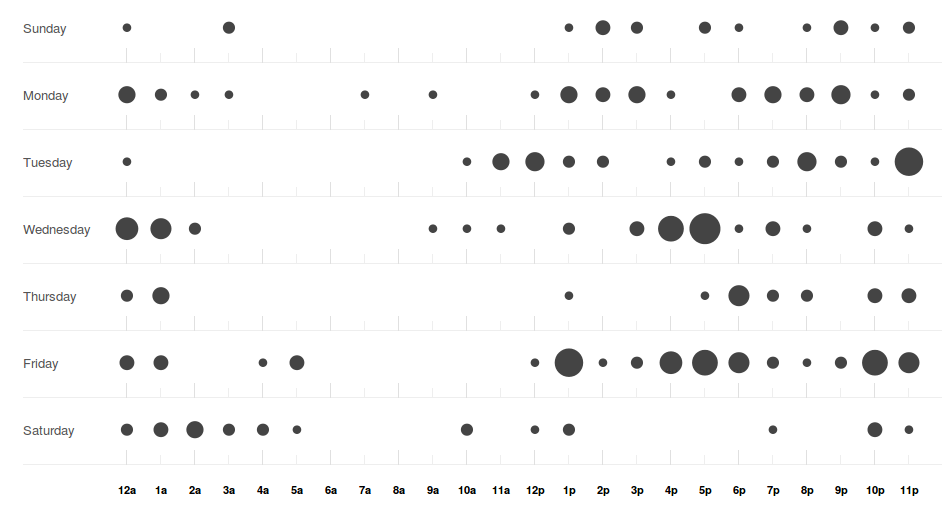
\includegraphics[scale=0.4]{img/punchcard.png}
\caption{Punchcard - Darstellung der Entwicklungszeiten}
\label{fig:punchcard}
\end{figure}
 
\chapter{Diskussion}
In der letzten Wochen vor der Abgabe der Arbeit waren wir sehr begeistert von unserem Spiel. Klar kennen wir die Schwächen und hätten gerne mehr Ideen verwirklicht und vor allem noch mehr Levels erstellt. Wir dürfen aber durchaus behaupten, dass wir in der verfügbaren Zeit, unser ambitioniertes Ziel erreichten und während dem Projekt nichts taten, was uns später blockierte oder unsere Ziele gar gefährdeten. Wir waren während der ganzen Arbeit immer sehr motiviert. Die Zusammenarbeit im Team machte uns sehr Spass und funktionierte jederzeit einwandfrei. 


\chapter{Mögliche Erweiterungen / Ausblick}
Wir wissen, dass wir noch einige Schritte von einem kompletten Game entfernt sind. Es fehlen noch verschiedene Levels. Wir möchten auch noch Gegner einbauen, wie zum Beispiel herumlaufende Hunde, die den Einbrecher entdecken könnten. Wir möchten auch, dass der Schallpegel erhöht wird, im Falle von einer Kollision mit einer Mauer.     
\\
Es wäre auch möglich, dass man den Dieb noch auf der Flucht spielen muss. So dass, wenn der Schallpegel überschritten ist, man noch wenig Zeit hat, um vor der Polizei zu fliehen.
\\      
\\     
Wir werden weiterhin an diesem Spiel schreiben, weil uns das Spiel und dessen Programmierung sehr gefällt, aber auch, weil uns der Ehrgeiz gefasst hat: Wir wollen ein richtiges Spiel zusammenstellen. Unsere Wunschvorstellung wäre, dass wir es dann einmal auf eine Online Spieleplattform stellen könnten, so dass es dann auch von anderen Leuten gespielt wird.


\clearpage
\mbox{}\clearpage
\pagenumbering{Roman}
\part{Anhang}
\listoffigures

\clearpage

\addcontentsline{toc}{chapter}{Literatur}
\printbibliography

\clearpage

\addcontentsline{toc}{chapter}{Antiplagiatserklärung}
\chapter*{Antiplagiatserklärung}
Wir versichern hiermit, dass wir die vorliegende Arbeit, inklusive des entstandenen Spiels, sämtlichen Programmcodes und Dokumentationen
selbständig und ohne fremde, undeklarierte Hilfe erstellten. Sämtliche Quellen, die zur Erstellung
der Arbeit verwendet wurden, wurden in der Literaturliste aufgeführt.
\\\\\\
\textbf{Aarau, der \today}\\

% Hier kommen die Unterschriften hin
\vspace{1 cm}
\begin{tabular}{p{5cm}p{.5cm}l}
\dotfill \\
\begin{center}
Gabriel Gavrilas

\end{center}\end{tabular}%
\hfill
\begin{tabular}{p{5cm}p{.5cm}l}
\dotfill \\
\begin{center}
Jan Kunzmann

\end{center}\end{tabular}%
\hfill
\begin{tabular}{p{5cm}p{.5cm}l}
\dotfill \\
\begin{center}
Patrick Eigensatz
\end{center}
\end{tabular}%
\\

\chapter*{Der Quellcode zum Spiel}
\addcontentsline{toc}{chapter}{Der Quellcode zum Spiel}
In unserer Arbeit ist ein ganzes Computerspiel entstanden. Vom Spiel ist der Quellcode natürlich die grösste Arbeit.
Unser Spiel ist in 26 verschiedenen Dateien aufgeteilt. Es existieren Quellcodedateien (\textit{.cpp}) und auch Headerdateien (\textit{.h}).\\
\\
Zählt man nur unseren reinen Code, kommt man auf 1250 Zeilen. Dazu kommen noch 275
Zeilen Kommentare ($\widehat{=}\,18\%$), sowie 475 leere Zeilen, die zur Strukturierung und Lesbarkeit des Codes beitragen.\\
\\
Den Quellcode ist auf den nächsten Seiten zu finden. Um Papier zu sparen wurde der Code auf zwei Seiten pro Blatt
gedruckt.

\end{document}







